\documentclass[main.tex]{subfiles}
 
\begin{document}
\chapterimage{band1.jpg}
\chapter{Introduction}

\section{ESP-Jumpstart: Build ESP32 Products Fast}\index{ESP32: Build ESP32 Products Fast}

Building production-ready firmware can be hard. It involves multiple questions and decisions about the best ways of doing things. It involves building phone applications, and integrating cloud agents to get all the features done. What if there was a ready reference, a known set of best steps, gathered from previous experience of others, that you could jumpstart with?

ESP-Jumpstart is focused on building \textit{products} on ESP32. It is a quick-way to get started into your product development process. ESP-Jumpstart builds a fully functional, ready to deploy "Smart Power Outlet" in a sequence of incremental tutorial steps. Each step addresses either a user-workflow or a developer workflow. Each step is an application built with ESP-IDF, ESP32's software development framework.

\begin{figure}[h!]
    \centering
    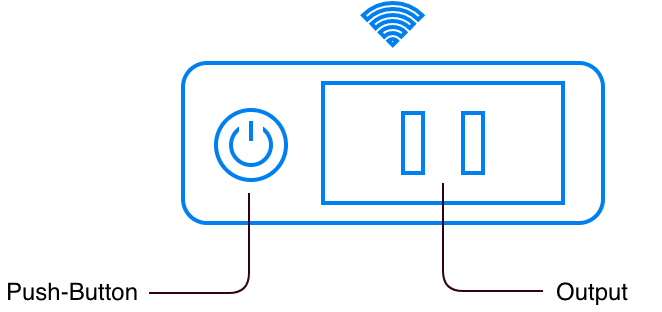
\includegraphics[scale=0.4]{../../_static/jumpstart-outlet.png}
    \caption{Smart Power Outlet}
    \label{fig:power_outlet}
\end{figure}

The ESP-Jumpstart's Smart Power Outlet firmware assumes the device has one input push-button, and one GPIO output. It implements the following commonly required functionality.

\begin{itemize}
  \item Allows and end-user to configure their home Wi-Fi network through phone applications (iOS/Android)
  \item Switch on or off the GPIO output
  \item Use a push-button to physically toggle this output
  \item Allow remote control of this output through a cloud
  \item Implement over-the-air (OTA) firmware upgrade
  \item Perform \textit{Reset to Factory} settings on long-press of the push-button
\end{itemize}

Once you are familiar with ESP-Jumpstart, building your production firmware, is a matter of replacing the power-outlet's device driver, with your device driver (bulb, washing machine).

\begin{figure}[h!]
    \centering
    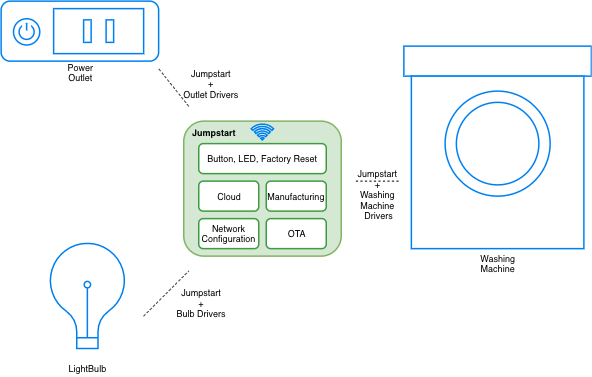
\includegraphics[scale=0.7]{../../_static/jumpstart-outlet-blocks.png}
    \caption{Jumpstart Applicability}
    \label{fig:jumpstart_applicability}
\end{figure}

You will require the following to get started:
\begin{itemize}
\item An ESP32 development kit: ESP32-DevKit-C \url{https://www.espressif.com/en/products/hardware/esp32-devkitc/overview} available through your closest store. You could also use any other ESP32 development board if you already have one.
\item A Development host setup (Windows, Linux or Mac) that will be used for development.
\end{itemize}

\section{For the Restless}\index{For the Restless}
If you are familiar with Espressif's hardware and/or embedded systems, and are looking for a production-reference without the incremental steps, you can do the following: 

\begin{enumerate}
    \item Directly use the final application in ESP-Jumpstart
    \item If you don't have a cloud account, configure your AWS IoT Cloud configuration as mentioned in Section \ref{sec:aws_cloud}
    \item Create the manufacturing configuration file for your device's unique cloud credentials, based on the instructions provided in Section \ref{sec:gen_factory_data} and flash it at the appropriate location
    \item Build, flash and boot up the firmware image as you usually do
    \item Use the reference phone-app (iOS/Android) libraries for building your phone applications. Or use the reference application to try things out as discussed in Section \ref{sec:unified_prov}
    \item Use the commands discussed in Section \ref{sec:aws_cloud} for remote control
    \item Now that you have this functional, modify to work with your driver
\end{enumerate}

\end{document}
